\subsection{OR}
    The OR gate represents the logical disjunction ($\lor$) from mathematical logic, and its operation can be represented as $\text{OR}(A, B) = A + B$, where $A$ and $B$ are the input signals. \\
    The circuitry of an OR gate involves multiple transistors arranged in parallel. 
    For a two-input OR gate, two transistors are connected in parallel, as shown in Figure \ref{fig:OR_circuit}. \\
    If either or both inputs are high (1), at least one of the transistors conducts, providing a low-resistance path from the power supply to the output, resulting in a high output (1). 
    Only when both inputs are low (0) will both transistors be off, causing the output to be pulled to a low state (0).
    This behavior is consistent with the OR gate's truth table shown in Table \ref{tab:OR_table}. \\
    The symbol for the OR gate is shown in Figure \ref{fig:OR_sym}.

    \begin{figure}[H]
	    \centering
	    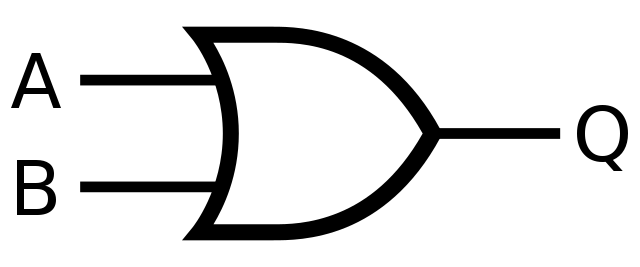
\includegraphics[width=0.3\textwidth]{figures/symbols/OR.png}
	    \caption{OR symbol.}
	    \label{fig:OR_sym} 
	\end{figure}

    \begin{figure}[H]   
        \begin{minipage}{0.5\textwidth}
            \centering
            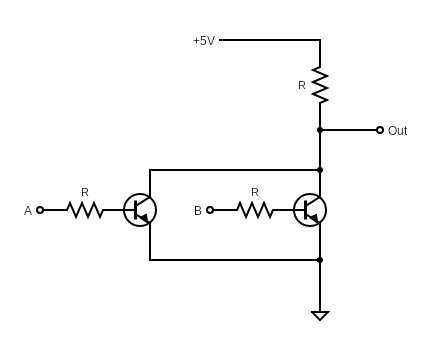
\includegraphics[width=1.1\textwidth]{figures/circuits/OR.png}
            \captionof{figure}{OR schematic circuit.} 
            \label{fig:OR_circuit} 
        \end{minipage}
        \begin{minipage}{0.5\textwidth}
            \centering
            \captionof{table}{OR truth table.}
            \begin{tabular}{|c|c|c|}
                \hline
                Input A & Input B & Output \\
                \hline
                0 & 0 & 0 \\
                0 & 1 & 1 \\
                1 & 0 & 1 \\
                1 & 1 & 1 \\
                \hline
            \end{tabular}
            \label{tab:OR_table}
        \end{minipage}
	\end{figure}

    \noindent
    The following photographs show the OR gate built in the laboratory and its behavior.
    \begin{figure}[H]
        \centering

        \begin{subfigure}{0.45\textwidth}
            \centering
            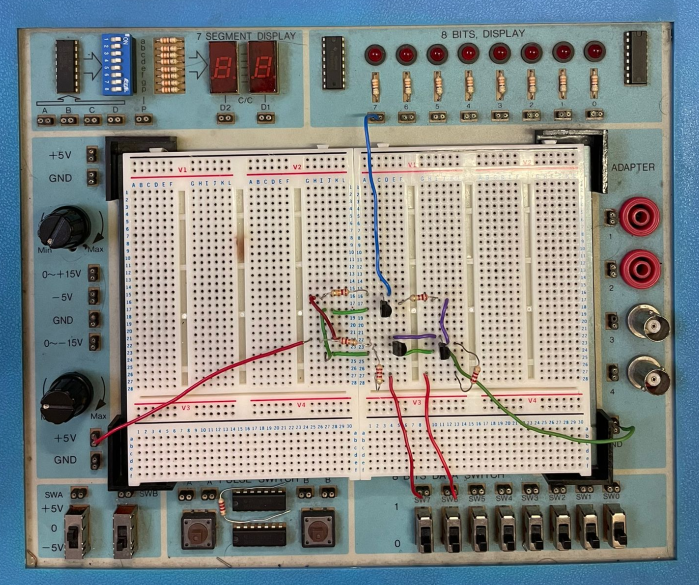
\includegraphics[width=\linewidth]{figures/photos/OR/00.png}
            \caption{A = 0, B = 0}
        \end{subfigure}
        \hfill
        \begin{subfigure}{0.45\textwidth}
            \centering
            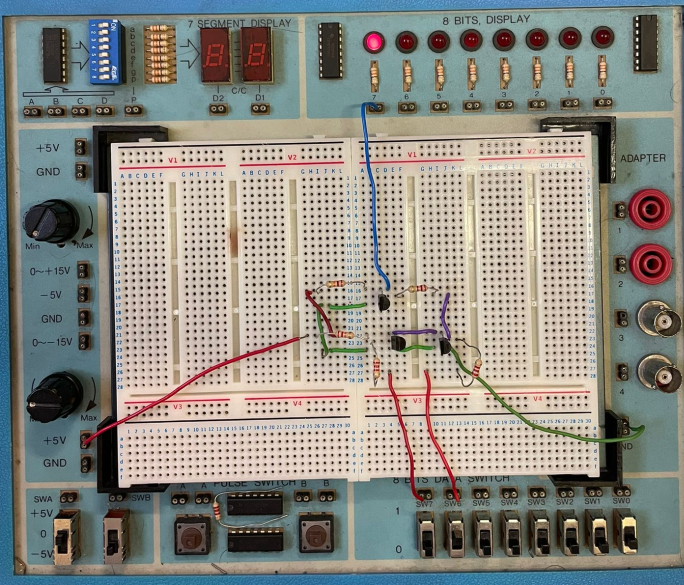
\includegraphics[width=\linewidth]{figures/photos/OR/01.png}
            \caption{A = 0, B = 1}
        \end{subfigure}

        \vspace{1cm} % Adjust vertical space between rows

        \begin{subfigure}{0.45\textwidth}
            \centering
            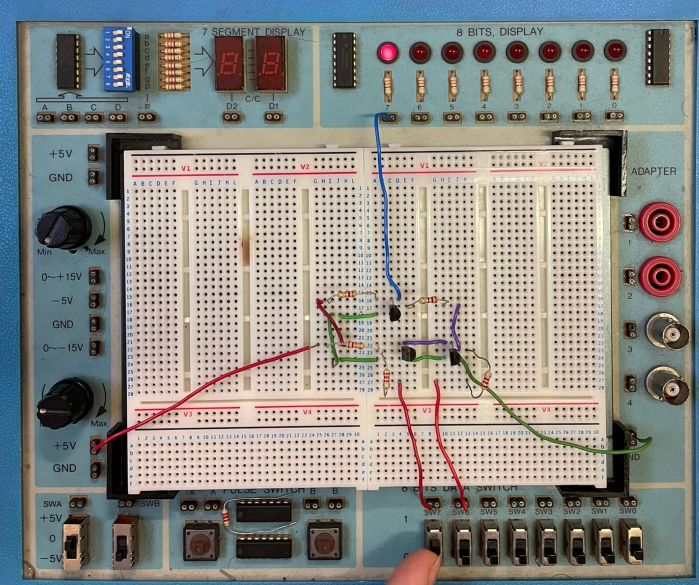
\includegraphics[width=\linewidth]{figures/photos/OR/10.png}
            \caption{A = 1, B = 0}
        \end{subfigure}
        \hfill
        \begin{subfigure}{0.45\textwidth}
            \centering
            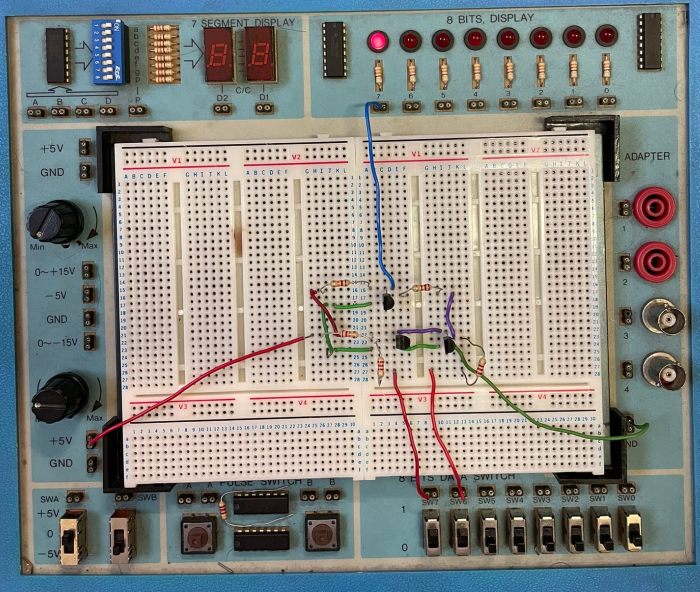
\includegraphics[width=\linewidth]{figures/photos/OR/11.png}
            \caption{A = 1, B = 1}
        \end{subfigure}

        \caption{OR gate constructed in the laboratory.}
        \label{fig:OR_photos}
    \end{figure}
